\chapter{引言}

\section{项目背景}

Online Judge 系统(简称OJ)是一个在线的判题系统。用户可以在线提交程序多种程序(如C、C++、Pascal)源代码,系统对源代码进行编译和执行,并通过预先设计的测试数据来检验程序源代码的正确性。

Online Judge 系统最初使用于ACM-ICPC国际大学生程序设计竞赛和OI信息学奥林匹克竞赛中的自动判题和排名。现广泛应用于世界各地高校学生程序设计的训练、参赛队员的训练和选拔、各种程序设计竞赛以及数据结构和算法的学习和作业的自动提交判断中。如北航的 AC 编程平台已服务于《程序设计基础(C 语言)》、《大学计算机基础(Python 语言)》等许多课程。这样的评测平台有助于提高学生的编程能力。

但是,传统的 OJ 平台仍然存在着许多局限性:它通常只能以黑盒测试的形式, 反馈通过的测试用例的数量,而与其代码质量无关; 它通常也仅能对单文件的项目进行测评, 难以承载一个项目的评测。 目前市场上虽然有极少数 OJ,如 CourseGrading、 rurikara 支持多文件的测评。 但这些平台在遇到多个用户同时评测时, 由于评测项目的开销过于庞大, 常常会发生等待和卡死的情况,并发性不佳。

\begin{figure}[H]
    \centering
    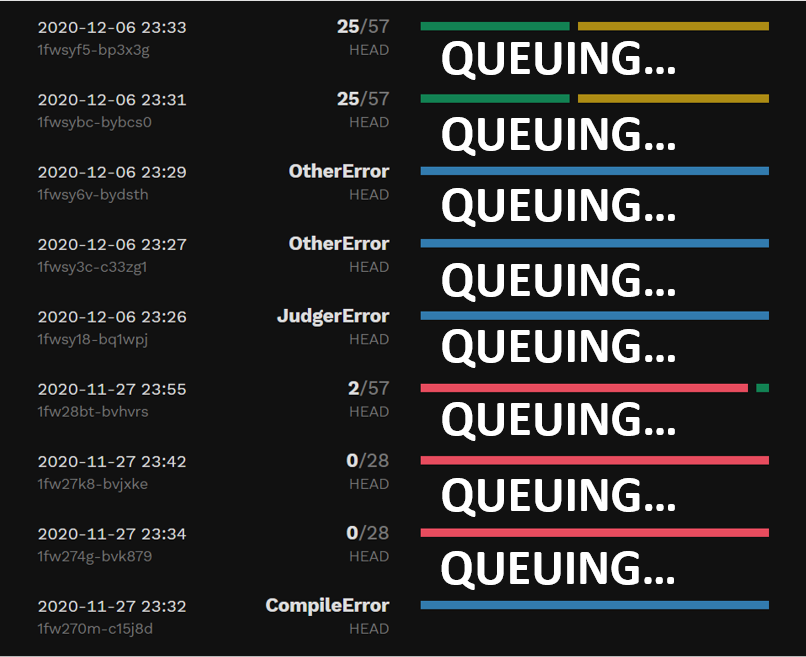
\includegraphics[width=0.7\textwidth]{figure/queuing.png}
    \caption{\textbf{传统评测机出现了卡死等待的情况}}
    \label{fig:queuing}
\end{figure}

开发这个项目的原因来自于课程的需求,如软件学院的《面向对象程序设计》课程,其中一项需要反复迭代的 Java 大作业的评测需要通过上百条命令的黑箱测试。对学生而言,一条命令一条命令地在终端中输入,并通过人眼进行与期望输出的比较过于费时费力;对老师和助教而言,几百人的学生作业也不可能人工地进行代码编译、运行并手动执行输入命令。北航的 AC 编程平台只支持单文件的评测,无法应用于含 package 包,有相对复杂的目录结构的 Java 程序项目之中;其反馈的结果只有正确和错误两项,没有调试信息,学生只能“瞎”尝试,不利于语言的学习。鉴于市场上已有的在线评测系统均不能满足类似课程的需求,因此,为了解决学生、助教和老师在评判作业和使用其他同类评测平台时的痛点开发了该程序评测系统。

\section{项目概述}

本项目旨在为许多学习程序语言的课堂以及希望学习编程的用户提供服务。通过使用该评测系统,用户能查看特定方向的教程,并进行练习、评测,平台也能根据评测结果的反馈和大数据的统计分析结果作出做题推荐。本平台希望能借助这些功能和设计思路快速提升用户的编程能力。

这是一款支持多人同时在线使用的分布式程序评测系统。系统内置了相当多的编程题目,用户可在其中选择题目练习,并通过本评测系统评判和检测程序的正确性。每当用户评测其编写的程序后,所有的评测数据会持久化地保存于远程数据库。系统还能够针对性地对个人以及多人给出基于评测大数据的统计分析结果,给出学习建议和推荐题目,帮助用户快速提高编程能力。对于老师和助教,该系统也支持编辑题目、提交测试样例中的标准输入与输出等。

通过自定义编译和运行代码的配置,该评测系统完整地支持了 Java、Python、C、C++等各种编程语言\cite{wu2012development}。目前该评测机也支持 Windows、Linux、Mac OS 等全平台使用。

与北航的 AC 编程平台相比,本系统额外支持了含多文件、多目录的程序评测,支持的编程语言也远远超过了 AC 编程平台。此外,与传统的在线评测平台,如 LeetCode、牛客网等相比,本程序评测系统创新性地将需要消耗大量算力的程序编译和执行过程分布式地分散到了用户的本地电脑主机,大幅减轻了远程服务器的算力要求。非常适合成本非常有限的课堂环境的教学之中。

\section{项目创新点与先进性}

\begin{enumerate}
    \item 将算力分布到用户的本地主机,避免了算力集中导致的资源浪费。去中心化,创新性地使用到了分布式并行计算思想。
    \item 基于 Electron 开发,支持跨平台使用,该评测系统在 Windows、Linux 和 Mac OS 等操作系统上均可使用。
    \item 安装简单,只需指定安装目录即可使用,界面友好易操作。
    \item 支持对含多文件,有复杂目录的程序进行评测。
    \item 支持对 Java、Python、C、C++、Go 等各种语言的评测。可自定义配置编译和运行的命令,以支持任何编程语言。
    \item 自定义设置标准输入和输出,支持多评测文件,多点一起评测,可设置各点的权重。
    \item 完善的评测结果判断和分析:可判断是否编译失败、程序运行超时、运行时发生异常、与期望输出不符等。
    \item 智能推荐给用户做最适合自己的题目,提升学习体验。
\end{enumerate}

\section{项目难点与解决方案}

\begin{enumerate}
    \item \textbf{如何向目标程序调用编译、执行命令?}\\
          利用Nodejs的多进程相关API,创建子进程进行操作。
    \item \textbf{如何将输入数据传给目标程序,并获取到目标程序的输出?}\\
          将 I/O 的输入输出进行重定向。
    \item \textbf{如何判断编译成功或失败?}\\
          获取编译程序的返回值。若为 0,编译成功;若不为 0,编译失败,将不会进行后续的评测工作。
    \item \textbf{如何判断程序超时?}\\
          利用Nodejs的多进程相关API,设定子进程的运行时间限制。
    \item \textbf{如何实现跨平台构建?}\\
          在工作流中将构建分为Windows构建、Linux构建、Mac OS构建三个任务,利用Github Actions进行自动构建。
\end{enumerate}